\documentclass[12pt,a4paper]{article}

% Packages
\usepackage[utf8]{inputenc}
\usepackage[T1]{fontenc}
\usepackage{amsmath}
\usepackage{amssymb}
\usepackage{graphicx}
\usepackage[margin=1in]{geometry}
\usepackage{setspace}
\usepackage{hyperref}
\usepackage{cite}
\usepackage{natbib}
\usepackage{float}

% Document settings
\onehalfspacing
\setlength{\parindent}{0.5in}
\setlength{\parskip}{0pt}


\title{
    
\includegraphics[width=1.5in]{logo.png}\\[2.5mm]
    \textbf{TRIBHUVAN UNIVERSITY} \\
    \large \textbf{INSTITUTE OF ENGINEERING} \\
    \large \textbf{PULCHOWK CAMPUS} \\
    \vspace{1cm}
    \large \textbf{A \\Project Report\\ On} \\
    \vspace{1cm}
    \large\textbf{A Modular Memory Management Architecture for Context-Aware Large Language Models}
    \vspace{.5cm}
}

\author{
    \textbf{SUBMITTED BY:} \\
    Aayush Ojha (079BCT005) \\
    Ankit Raj Mehta (079BCT018) \\
    Ashish Pandey (079BCT023)
}

\date{
    \vspace{1cm}
    \textbf{SUBMITTED TO:} \\
    {DEPARTMENT OF ELECTRONICS AND COMPUTER ENGINEERING} \\
    \vspace{2cm}
    March, 2026
}


\begin{document}

\maketitle
\thispagestyle{empty}
\newpage

\pagenumbering{roman}
\setcounter{page}{1}


\newpage
\section*{Page of Approval}
\addcontentsline{toc}{section}{Page of Approval}
\vspace{1.5cm}
\begin{center}
\uppercase{
Tribhuvan University\\
Institute of Engineering\\
Pulchowk Campus\\
Department of Electronics and Computer Engineering
    }
\end{center}
\vspace{.5cm}
The undersigned certifies that they have read and recommended to the Institute of Engineering for acceptance of a project report entitled \textbf{"MemBlocks"} submitted by \textbf{Ashish Pandey (079BCT023)} in partial fulfillment of the requirements for the Bachelor's degree in Electronics \& Computer Engineering.\\

\vspace{1cm}
\begin{minipage}{.5\textwidth}
    \raggedright
    .............................\\
    Supervisor\\
    \textbf{Full Name}\\
    Designation\\
    Department of Electronics and Computer Engineering,\\
    Pulchowk Campus, IOE, TU.\\
\end{minipage}%
\begin{minipage}{0.5\textwidth}
    \raggedleft
    .............................\\
    External examiner\\
    \textbf{Full Name}\\
    Assistant Professor\\
    Department of Electronics and Computer Engineering,\\
    Pulchowk Campus, IOE, TU.\\
\end{minipage}\\
\vspace{1.5cm}
\centerline{Date of approval:}

\newpage
\section*{Copyright}
\addcontentsline{toc}{section}{Copyright}
The author has agreed that the Library, Department of Electronics and Computer Engineering, Pulchowk Campus, and Institute of Engineering may make this report freely available for inspection. Moreover, the author has agreed that permission for extensive copying of this project report for scholarly purposes may be granted by the supervisors who supervised the work recorded herein or, in their absence, by the Head of the Department wherein the project report was done. It is understood that recognition will be given to the author of this report and the Department of Electronics and Computer Engineering, Pulchowk Campus, Institute of Engineering for any use of the material of this project report. Copying publication or the other use of this report for financial gain without the approval of to the Department of Electronics and Computer Engineering, Pulchowk Campus, Institute of Engineering, and the author's written permission is prohibited.\\
Request for permission to copy or to make any other use of the material in this report in whole or in part should be addressed to:\\

\vspace{1.5cm}
Head\\
Department of Electronics and Computer Engineering\\
Pulchowk Campus, Institute of Engineering, TU\\
Lalitpur, Nepal.


\newpage
\section*{Acknowledgement}
\addcontentsline{toc}{section}{Acknowledgement}

We would like to express their sincere gratitude to the \textbf{Department of Electronics and Computer Engineering} for providing the academic environment, resources, and guidance necessary for the successful completion of this project. We are thankful to the faculty members for their continuous support, constructive feedback, and encouragement throughout the course of this work. Their guidance and expertise have played a crucial role in shaping this project and enhancing our learning experience.
\clearpage


\section*{Abstract}
\addcontentsline{toc}{section}{Abstract}
MemBlocks is a modular memory architecture for Large Language Models (LLMs) that addresses fixed context windows and limitations of monolithic Retrieval-Augmented Generation systems. It organizes memory into independent, attachable blocks representing distinct domains such as personal, academic, and project contexts. Each block contains structured components including core attributes, semantic memory, and recursive summaries for compressed conversational state.

The system employs hybrid semantic and metadata-based retrieval to selectively assemble relevant context, reducing retrieval noise and improving scalability. Memory updates are performed through structured extraction, conflict resolution, and recursive summarization, allowing stored knowledge to remain coherent while reducing redundancy. The implementation emphasizes section-aware storage and retrieval behavior so that persistent facts, semantic memories, and compressed recent context contribute differently during response generation.

\textbf{Keywords:} Large Language Models, Memory Management, Retrieval-Augmented Generation, Modular Architecture, Context Management, AI Agents, Vector Databases, Semantic Memory

\clearpage



\tableofcontents

\addcontentsline{toc}{section}{List of Figures}
\listoffigures
\clearpage


\section*{Abbreviations}

\begin{description}

    \item[LLM] Large Language Model
    \item[LC] Long Context
    \item[LLMs] Large Language Models

    \item[RAG] Retrieval-Augmented Generation
    \item[RRF] Reciprocal Rank Fusion

    \item[MIRIX] Multi-Agent Memory System

    \item[NLP] Natural Language Processing

    \item[OS] Operating System

    \item[UX] User Experience

    \item[BM25] Best Matching 25 (ranking function)

    \item[HyDE] Hypothetical Document Embeddings

    \item[JSON] JavaScript Object Notation

    \item[XML] Extensible Markup Language

    \item[p95] 95th percentile
    \item[NOOP] No Operation
\end{description}
\clearpage

\clearpage
\pagenumbering{arabic}
\setcounter{page}{1}


\section{Introduction}

\subsection{Background}

Large Language Models (LLMs) are increasingly used in intelligent assistants, educational tools, enterprise systems, and productivity platforms. These systems depend on contextual information such as prior conversations, user preferences, domain knowledge, and documents to produce meaningful and accurate responses. However, LLMs do not possess persistent memory by default and operate within fixed context window limits, meaning they cannot continuously retain long-term information.

To address this limitation, modern AI systems incorporate external memory techniques such as chat history storage, Retrieval-Augmented Generation (RAG), and vector databases. While these approaches allow past information to be stored and retrieved, they typically treat memory as a single, centralized repository. As AI systems expand to support multi-domain usage and long-term interactions, this monolithic memory design becomes inefficient, difficult to manage, and prone to contextual conflicts.

Simultaneously, users now interact with AI systems in multiple roles  personal, academic, and professional creating the need for structured memory separation and better control over what information is used during interactions. This highlights the importance of designing a modular, scalable, and user-centric memory infrastructure for LLM-based agents.

\subsection{Problem Statement}

Despite advancements in LLM performance, memory management remains a major limitation at both system and user levels.

From the AI system perspective, LLMs have fixed context windows and cannot inherently maintain long-term or cross-session memory. External memory solutions such as RAG extend storage capacity but introduce several architectural challenges. Information is often stored in unified memory pools without clear separation between different contexts, causing retrieval noise where irrelevant information is returned alongside relevant data. Additionally, facts, conversation summaries, and documents are treated similarly, even though they require different storage and retrieval strategies. This lack of structural differentiation reduces retrieval efficiency and makes context management complex. Existing systems also lack built-in mechanisms for modular context switching, selective activation of memory, and organized composition of different knowledge sources.

From the user perspective, current memory systems provide limited control over how personal, academic, or professional information is organized and exposed to the AI model. Multiple aspects of a user's identity  preferences, work tasks, and learning materials  are often merged into a single memory space. This makes it difficult to separate knowledge domains and increases the possibility of irrelevant or sensitive information being retrieved during unrelated interactions. Users cannot easily specify which information should be active in a given conversation, resulting in unnecessary context being sent to the model, increased operational cost, and reduced response relevance.

Furthermore, switching between tasks or roles is not handled systematically. Context switching often depends on implicit assumptions by the system, leading to inconsistent behavior. The absence of modular memory isolation limits scalability, reliability, and user trust.

Therefore, the core issue is both architectural and user-centric: existing LLM memory mechanisms are monolithic and unstructured, whereas real-world AI usage requires modular, composable, and user-controlled memory systems capable of separating contexts, supporting multiple memory types, and enabling reliable context switching.

\subsection{Objectives}

The primary objective of this project is to design and implement a Modular Memory Management System for LLM agents, named MemBlocks, where contextual information is organized into independent, attachable memory blocks.

The specific objectives are:

\begin{enumerate}
    \item To design a modular memory block architecture where each block represents a separate context such as personal data, project knowledge, or learning material.
    
    \item To organize each memory block into structured sections, including core memory (essential facts), semantic memory (knowledge and events), and recursive summary (conversation compression and continuity).
    
    \item To enable dynamic attachment and detachment of memory blocks, so that only relevant contexts are active during a conversation.
    
    \item To provide user-level control over context exposure, allowing users to manage which memory blocks are used by the LLM.
    
    \item To implement intelligent retrieval mechanisms that understand query intent, search different memory sections using appropriate strategies, and reduce irrelevant context.
    
    \item To improve context relevance, scalability, and reliability compared to traditional monolithic memory systems.
\end{enumerate}

\subsection{Scope of the Project}

This project focuses on the design and implementation of a modular memory infrastructure layer for LLM-based conversational agents. The scope includes:

\begin{enumerate}
    \item Designing memory blocks and their internal structure,
    
    \item Implementing mechanisms to create, attach, detach, and manage memory blocks at runtime,
    
    \item Developing retrieval orchestration across multiple memory sections,
    
    \item Supporting user-level context control across memory blocks,
    
    \item Integrating with existing storage technologies such as vector databases,
    
    \item Demonstrating the system through a prototype conversational AI application.
\end{enumerate}

The project does not involve:

\begin{enumerate}
    \item Training new large language models,
    
    \item Developing new embedding or vector search algorithms,
    
    \item Building a full-scale commercial deployment.
\end{enumerate}

The primary contribution lies in memory architecture, modular organization, and user-centric context management, which are essential for scalable and practical AI systems.

\section{Literature Review}

The current landscape of Large Language Model (LLM) utility is increasingly defined by the transition from stateless, predictive text engines to stateful, autonomous agents capable of sustained interaction over extended temporal horizons \cite{luo2025large}. However, the foundational architecture of the transformer model presents a significant impediment to this transition: the finite context window. As interactions progress, the sequential nature of input processing necessitates the gradual displacement of historical data, leading to a phenomenon of ``digital amnesia'' that undermines personalization, continuity, and task-specific reliability \cite{liu2024lost}. While the industry has attempted to mitigate these constraints through Retrieval-Augmented Generation (RAG) and the expansion of context windows, these solutions often operate through indiscriminate data accumulation, failing to provide the granular control and modularity required for complex, multi-domain user identities \cite{li2025memos}. Through this section, we analyze the evolution of context management, the rise of agentic memory frameworks, and the necessity of a modular ``cartridge'' approach to memory.

\subsection{The Historical Trajectory of Statehood and Context Management}

The development of LLM memory systems has evolved through three distinct phases, each attempting to resolve the inherent tension between computational efficiency and context retention. Early conversational systems relied on history injection, where previous dialogue turns were simply prepended to the current prompt. Although straightforward, this strategy scales poorly due to the $O(n^2)$ time and space complexity of dot-product self-attention \cite{vaswani2017attention}, causing latency and token-level computation costs to grow rapidly as the conversation length increases.

The second phase saw the emergence of a dual-track strategy: Long Context (LC) expansion and Retrieval-Augmented Generation (RAG). Long Context models, exemplified by the 2024-2025 releases from Google \cite{reid2024gemini} and Anthropic, push the boundaries of the context window to millions of tokens, theoretically allowing the model to ``pre-load'' massive datasets directly into its working memory. Empirical evaluations demonstrate that LC strategies generally outperform RAG in tasks requiring holistic reasoning over static datasets, such as summarization or Wikipedia-based question answering \cite{li2024long}. However, LC is not a complete solution; it remains computationally expensive and often fails to differentiate between relevant and irrelevant information when the ``haystack'' of data becomes too large.

In parallel, RAG introduced a hybrid paradigm where generative capabilities are enhanced through real-time access to external vector databases. This allows for the dynamic querying of massive, evolving knowledge bases without overloading the immediate context window. Despite its utility, conventional RAG suffers from ``retrieval noise'', the tendency to retrieve outdated or semantically similar but contextually irrelevant information, and treats all stored data as an undifferentiated mass \cite{li2024retrieval}.

The third and most current phase involves the development of ``Agentic Memory,'' where memory is no longer a passive repository but an active, self-managed component of the agent's architecture. Systems such as MemGPT \cite{packer2023memgpt} (now Letta) and Mem0 \cite{chhikara2025mem0} have pioneered this approach, treating memory as a tiered system that the agent can autonomously edit, prune, and reorganize.

The evolution depicted in current research highlights a trend toward models that handle longer context windows while simultaneously integrating modular RAG methods to optimize efficiency. However, even as models like Claude 4 and GPT-5 offer improved long-term memory, they remain essentially ``black boxes'' from the user perspective, providing minimal control over how data is partitioned or exposed.

\subsection{Corporate Implementations}

The competitive landscape of 2024 and 2025 has seen major AI providers integrate persistence features directly into their flagship models. OpenAI's ``Memory'' feature, launched in early 2024, utilizes an accessible memory log that can be reviewed and edited by the user, representing a foundational step toward transparency. By mid-2025, this functionality was expanded to allow the system to reference all past conversations, significantly enhancing personalization across sessions.

Anthropic and Google have followed divergent paths. Google unified its Gemini brand, introducing memory features in early 2025 that allow the system to autonomously search through previous conversations to supplement current outputs. Anthropic, through its Claude ``Projects'' functionality, introduced a nascent form of modularity by separating project-specific memory from general saved memory, preventing cross-contamination of unrelated tasks.

Despite these advancements, these systems face systemic challenges in ``Context Isolation'' \cite{wu2024secgpt}. When a user's personal preferences, professional responsibilities, and ongoing study/work threads are merged into a single memory space, the risk of ``Context Leakage'' increases. For instance, documents or knowledge relevant to a user's personal life or academic study may be inadvertently surfaced during work-related interactions, or vice versa. In entrepreneurial or startup-oriented workflows, users are often forced to repeatedly re-explain the full scope of an idea in newly isolated conversations to avoid unintended context carryover from casual or personal chats, as the alternative risks contaminating professional queries with irrelevant or sensitive personal information. Furthermore, these systems lack a standardized mechanism for users to ``attach'' or ``detach'' specific knowledge modules. The memory extraction remains largely automated, driven by heuristics that the user cannot easily audit or override.

\subsection{The Shift to Agentic and Autonomous Memory}

Recent literature identifies a transition from passive RAG systems to ``Agentic Memory,'' where the agent actively manages its cognitive state through specialized tools and hierarchical structures.

\subsubsection{Letta (formerly MemGPT)}

Letta \cite{packer2023memgpt} implements a memory hierarchy inspired by virtual memory paging in operating systems. It partitions memory into ``Main Context'' (in-context) and ``External Context'' (out-of-context). The architecture utilizes Core Memory blocks, containing persona and human-specific facts, which the agent can update via tool calls like \texttt{memory\_insert} and \texttt{memory\_replace}. This allows the agent to maintain a persistent state despite the limitations of the fixed context window.

\subsubsection{Mem0}

Mem0 \cite{chhikara2025mem0} focuses on the dynamic extraction of salient facts rather than raw logs. It uses a two-phase pipeline, Extraction and Update, to keep the memory store coherent. When a new fact is identified, Mem0 performs conflict resolution (ADD, UPDATE, DELETE, or NOOP) to ensure the ``latest truth'' is preserved. This approach can reduce token consumption by up to 90\% compared to full-context methods. In particular, Mem0 claims to attain a 91\% lower p95 latency and saves more than 90\% token cost, thereby offering a compelling balance between advanced reasoning capabilities and practical deployment constraints.

\subsubsection{A-mem (Agentic Memory)}

Inspired by the Zettelkasten method, A-mem \cite{xu2025amem} organizes memory as an interconnected network of structured ``notes''.

\begin{enumerate}
    \item \textbf{Note Construction:} Each interaction is transformed into a note with metadata including keywords, tags, and a contextual description.
    
    \item \textbf{Link Generation:} The system establishes connections between notes based on semantic similarity and shared attributes.
    
    \item \textbf{Memory Evolution:} Integrating new memories triggers updates to existing historical notes, allowing the agent's ``world model'' to refine itself as knowledge evolves over time.
\end{enumerate}

\subsection{Modular Knowledge Structures: The MIRIX Framework}

A critical advancement in modularity is presented in the MIRIX (Multi-Agent Memory System) \cite{wang2025mirix} paper. MIRIX addresses the limitations of ``flat'' memory systems by segmenting information into six specialized, structured containers:

\begin{enumerate}
    \item \textbf{Core Memory:} Foundational user data and agent persona.
    \item \textbf{Episodic Memory:} Specific interaction sequences and event details.
    \item \textbf{Semantic Memory:} General facts and concept-based knowledge.
    \item \textbf{Procedural Memory:} Instructions and skills on how to perform tasks.
    \item \textbf{Resource Memory:} External documents and tool-related data.
    \item \textbf{Knowledge Vault:} A secure repository for sensitive information.
\end{enumerate}

By utilizing a multi-agent framework where each container is managed by a dedicated agent, MIRIX allows for parallel updates and more accurate retrieval. On the LOCOMO benchmark, MIRIX achieved 85.4\% accuracy, outperforming baselines by providing a structured organization that reduces reasoning overhead.

This ``Context Engineering'' allows agents to maintain the illusion of infinite context within a fixed window by intelligently swapping information in and out of the active reasoning space. A critical innovation in this framework is ``Sleep-time Compute,'' where secondary agents update the primary agent's memory blocks during idle periods, reducing the cognitive load on the main agent during active dialogue.

However, these existing frameworks, while powerful, are primarily developer-facing. From a user experience (UX) perspective, the ``Core Memory'' blocks remain largely opaque, and the agent's self-editing capabilities can lead to ``Memory Anchoring,'' where the agent becomes overly constrained by its own history and fails to provide the ``fresh-start'' reasoning requested by the user. Moreover, these do not natively support the user-led creation of independent memory ``containers'' that can be selectively attached to different conversations to prevent domain overlap.

\subsection{Privacy, Safety, and the Risks of Persistent Context}

Persistent memory introduces significant vulnerabilities, particularly context leakage. In multi-persona or multi-session environments, users often expect an AI to remember their preferences while simultaneously desiring transparency and control over what is ``seen'' \cite{ali2025understanding}.

\begin{enumerate}
    \item \textbf{Context Leakage and Misuse:} Agents can inadvertently exfiltrate private data across sessions. Malicious prompts can trick an agent into revealing sensitive healthcare records or implementation details stored in its memory module.
    
    \item \textbf{Inference-Time Risks:} Models can deduce sensitive traits (e.g., location or political leaning) from seemingly ordinary data.
    
    \item \textbf{The Need for Transparency:} Current systems provide limited mechanisms for users to see why an agent remembered a specific fact or to ``gate'' information before it enters the long-term bank. Users frequently find that their professional and personal contexts merge, leading to inconsistent outputs and reduced privacy.
\end{enumerate}

\section{Methodology}

This chapter documents the methodology used to implement the MemBlocks system and the resulting operational design. The implemented architecture addresses fundamental limitations in current Large Language Model (LLM) memory systems through a modular, hierarchical approach to context management. Unlike traditional Retrieval-Augmented Generation (RAG) systems that treat all information uniformly in a single vector database, or systems like MemGPT and Mem0 that provide limited memory differentiation, MemBlocks implements distinct memory containers, section-specific retrieval, and structured update workflows. The following subsections describe the executed architecture, algorithmic workflows, data structures, and implementation technologies that support composable, context-aware memory management for AI agents.

\subsection{System Architecture}

The MemBlocks architecture follows a layered design that separates concerns between long-term memory storage, retrieval processing, and active conversational context management. Figure~\ref{fig:memBlocks_diagram1} shows this flow as a memory space with multiple containers connected to retrieval, update, and conversation components.

Memory Block Repositories serve as independent storage units, each maintaining its own organization and access semantics. At runtime, only attached containers participate in retrieval and updates, while detached containers remain isolated. Within an attached container, the implemented sections are Core Memory, Semantic Memory, and Recursive Summary. This sectioned organization avoids mixing persistent profile facts, query-relevant semantic memories, and compressed recent context in a single undifferentiated store.

The retrieval layer bridges long-term memory and the conversational LLM. As shown in Figure~\ref{fig:smart_retriver}, the query is expanded, embedded, and searched through hybrid retrieval, followed by RRF fusion and reranking. Core Memory and Recursive Summary are injected directly into the system prompt, while semantic memories are ranked and truncated to top-$k$ before assembly. This keeps the prompt compact while preserving high-value context.

The update path is event-driven from conversation history. When the sliding window reaches the configured limit, the system captures the current message window and triggers three coordinated update branches (Figure~\ref{fig:update_agent}): Core Memory evaluation, Semantic Memory extraction with conflict resolution, and Recursive Summary regeneration. Outputs from all branches are persisted back to storage, after which the active message window is trimmed to preserve short-term continuity.

Finally, the conversational LLM receives the assembled context (core + recursive summary + ranked semantic memories + recent turns + current input) and produces the response used for the next cycle.

\subsection{Memory Container Structure and Metadata}

Each memory container represents an independent knowledge domain with its own storage backend and retrieval semantics. Container-level metadata governs access patterns, update permissions, and semantic scope.

\subsubsection{Container Metadata Schema}

Every container maintains the following metadata fields that inform retrieval and update logic:

\begin{itemize}
    \item \textbf{container\_id:} Unique identifier enabling cross-container references and access control.
    
    \item \textbf{user\_id:} Associates the container with its owner account.
    
    \item \textbf{Container Definition:} A natural language description provided by the user that defines the intended purpose, semantic scope, or domain of the container. 
    
    \item \textbf{Creation and Usage Metadata:} Timestamps and access patterns tracking container lifecycle, last modification time, and usage frequency for optimization purposes.
\end{itemize}


\subsection{Memory Section Implementations}

Each container partitions its content into three implemented sections, each optimized for different information types and access patterns.

Resource memory is reserved for future implementation and is not part of the shipped memory section pipeline in the current project scope.

\subsubsection{Core Memory Section}

The Core Memory section stores high-priority, persistent information structured into two blocks: persona and human. The persona block encodes the agent's identity, behavioral guidelines, and interaction style. The human block contains enduring facts about the user, such as name, occupation, preferences, and self-identifying attributes. Core Memory content is injected into every LLM interaction via system prompts, ensuring these foundational facts persistently influence agent behavior.

\textbf{Reading Path.} On each interaction, the system constructs a prompt segment incorporating Core Memory.

\textbf{Writing Path.} Updates to Core Memory follow a conservative protocol. After a set of conversation exchanges, the Core Extraction Workflow evaluates whether the interaction contains Core-eligible information. The evaluation workflow explicitly constrains the agent to store only explicit, long-term, user information, preventing inference-based pollution of Core Memory. The workflow instructs the LLM to output a JSON structure indicating whether an update should occur and, if so, the revised persona and human blocks.

Core memory is manually defined to stay concise during each evaluation pass.

\subsubsection{Semantic Memory Section}

The Semantic Memory section stores extracted events, facts, and opinions about the user or the world. Each memory item includes key metadata such as type, timestamp, source, confidence, and entities to support efficient querying, reasoning, and temporal tracking.

\textbf{Data Model.} Each memory entry $m_i$ comprises the following fields:

\begin{itemize}
    \item $c_i$ (content): One-sentence summarized contextual description designed to evolve as new information arrives.
    
    \item $t_i$ (timestamp): Temporal marker enabling recency-based retrieval.
        
    \item $G_i$ (keywords): Categorical tags including domain tags (e.g., ``programming'', ``AI''), functional tags (e.g., ``optimization'', ``debugging''), and memory-nature tags (``fact'', ``event'', ``opinion'').
    
    \item $e_i$ (embedding): Dense vector representation generated from the concatenation of $c_i$, $K_i$, $G_i$, and $X_i$.
    
    \item \textbf{type:} Classification as fact, event, or opinion.
    
    \item \textbf{confidence:} Numeric score indicating reliability.
    
    \item \textbf{source:} Origin of the information (user-provided, inferred, external).
    
    \item \textbf{entities:} Named entities and domain concepts extracted from the content.
\end{itemize}

Additionally, each memory maintains metadata including memory\_id, usage timestamps, status flags, and message\_ids linking the memory to source conversation turns.

\textbf{Memory Addition Workflow For Semantic Memory.} When a new interaction $I_i$ occurs at time $t_i$, the system executes a five-step storage pipeline:

\begin{enumerate}
    \item \textbf{Structured Note Construction.} An LLM processes the interaction using the Semantic Extraction Workflow to generate keywords $K_i$, contextual description $c_i$, type classification, and entities. This structured extraction ensures consistent indexing across all memory entries.
    
    \item \textbf{Vector Embedding Generation.} The system concatenates $c_i$, $K_i$, and $X_i$ into a single text representation and passes it through an embedding model. This embedding model generates a dense vector $e_i$ suitable for efficient similarity search in the Qdrant vector database.
    
    \item \textbf{Semantic Candidate Retrieval.} The system queries Qdrant to compute similarity between $e_i$ and existing semantic memory embeddings. The top-$k$ most similar memories (configured in the service layer; default small candidate set) are retrieved as conflict candidates.
    
    \item \textbf{Conflict Resolution Decision.} The new memory proposal and candidate memories are passed to the LLM via the Memory Resolution Workflow. The model decides operations for the new candidate (ADD or NONE) and for each existing candidate (UPDATE, DELETE, or NONE), based on semantic overlap, contradiction, and specificity.
    
    \item \textbf{Storage Execution.} The decided operations are executed on the vector store: ADD inserts a new point, UPDATE rewrites the existing point with refreshed payload and embeddings, DELETE removes contradicted/superseded entries, and NONE performs no write. If the memory resolution fails, the pipeline falls back to direct ADD so memory ingestion does not halt.
\end{enumerate}

This storage workflow combines structured extraction, candidate retrieval, conflict adjudication, and deterministic write execution in one pipeline. Compared with flat append-only memory strategies, it reduces duplicate entries and keeps memory state aligned with newer evidence.

\subsubsection{Recursive Summary Section}

The Recursive Summary section implements a progressive compression mechanism for the recent conversation state. Recursive Summary focuses on intermediate-term context, recent goals, decisions, and unresolved threads that are too transient for permanent storage but too important to lose when the sliding window evicts messages.

\textbf{Trigger Conditions.} Recursive Summary updates trigger when conversation tokens exceed a threshold (typically 70-80\% of the LLM's context window). This threshold-based approach ensures the summary remains current without imposing update overhead on every message exchange.

\textbf{Reading Path.} On each LLM invocation, the current summary is injected into the system prompt:

\begin{verbatim}
<recursive_summary>
  {{summary}}
</recursive_summary>
\end{verbatim}

This placement ensures the LLM has access to recent contextual continuity without requiring full message history.

\textbf{Writing Path.} When the trigger condition activates, the system invokes an LLM with the Recursive Summary Workflow, providing the existing summary $S_{old}$ and new messages since the last update $\Delta C$. The LLM produces an updated summary $S_{new}$ that compresses repetition, preserves high-level goals and unresolved questions, and removes resolved details.

\subsection{Agentic Decision Logic Workflows}

The MemBlocks system relies heavily on carefully engineered workflows to guide LLM behavior in memory operations. This section details the primary workflows that drive core updates, structured note construction, memory resolution, and recursive summarization. Each workflow incorporates explicit constraints, output format specifications, and decision frameworks that ensure consistent, high-quality memory management.

\subsubsection{Core Extraction Workflow}

The Core Extraction Workflow evaluates whether recent interactions contain new persistent, long-term facts about the user or the agent's persona. It ensures that only explicit constraints, preferences, or core identity traits are saved, preventing short-term inference from polluting the core memory.

\subsubsection{Semantic Extraction Workflow}

The Semantic Extraction Workflow converts raw user queries into structured memory entries for embedding and retrieval. It guides the LLM to extract information for three purposes: hybrid retrieval, memory linking, and future refinement. Keywords must be salient, domain-specific, non-redundant, and free of generic verbs or filler. Context is captured in a single sentence summarizing the topic, supporting recursive evolution. Tags indicate domain, function, and memory nature, avoiding redundancy or over-specificity. Output is strictly formatted in JSON to enable reliable downstream processing.

\subsubsection{Memory Resolution Workflow}

The Memory Resolution Workflow manages integration of new information into existing memory by receiving a proposed memory from earlier extraction and a candidate set of semantically similar stored memories. It outputs structured JSON decisions with operation-level control: new memory can be ADD or NONE, while existing candidates can be UPDATE, DELETE, or NONE. This keeps deduplication and contradiction handling explicit and executable by the storage layer.

\subsubsection{Recursive Summary Workflow}

The Recursive Summary Workflow handles the recursive summarization of conversation by updating the previous summary with new messages while preserving essential context. It instructs the LLM to retain high-level goals, decisions, commitments, constraints, and unresolved actions, while removing resolved tasks, repetitive details, and obsolete context. Critical constraints prevent fabricating facts, storing personal or long-term user attributes, or duplicating content from Core or Semantic memory. The workflow produces a structured JSON output containing an updated\_summary field, ensuring deterministic integration of the compressed conversational context into the system.

\subsection{Retrieval Strategy and Context Assembly}

The MemBlocks retrieval strategy implements a multi-stage process that combines container selection, section-specific retrieval, and ranking to assemble relevant context for LLM invocation. This approach departs from monolithic RAG systems that perform flat semantic search across all stored content.

\subsubsection{Section-Specific Retrieval}

Within activated containers, retrieval proceeds section by section:

\textbf{Core Memory Retrieval.} Core Memory is always included in full, as it contains high-priority persistent information that should influence every interaction. No ranking or filtering applies to Core Memory; the entire persona and human blocks are injected into the system prompt.

\textbf{Semantic Memory Retrieval.} Retrieval from this section uses a hybrid path over memory embeddings. The system first performs query enhancement (expanded queries and hypothetical answer paragraphs), then embeds these query variants and searches Qdrant using dense and sparse retrieval. Candidate sets are fused using Reciprocal Rank Fusion (RRF), deduplicated, and reranked before the final top-$k$ semantic memories are passed forward to context assembly.

\textbf{Recursive Summary Retrieval.} The current Recursive Summary is always included in the system prompt, providing recent conversational continuity. No ranking or filtering applies; the entire summary is injected.


\subsubsection{Context Assembly}

After retrieval and ranking, the system assembles the final context for LLM invocation. The assembly follows a structured template that delineates memory sources: Core Memory first, Recursive Summary second, ranked semantic memories next, then recent sliding-window turns, followed by the current user input. This order preserves persistent identity/context priors while prioritizing query-relevant evidence for the current turn.

\subsection{Library Exposed Methods and Interfaces}

The MemBlocks library is designed as a memory management layer that can be integrated into any existing LLM orchestration system. It intentionally abstracts the complexity of database connections, hybrid search, and background agentic processing by exposing a clean, developer-friendly Python API. Below are the primary interaction points available through the \texttt{MemBlocksClient} interface.

\subsubsection{Client Initialization and Configuration}
Developers interface with the system primarily through the \texttt{MemBlocksClient}. It accepts a configuration object (\texttt{MemBlocksConfig}) that dictates database endpoints, embedding models, and granular LLM settings. This ensures the client remains agnostic to the underlying infrastructure while wiring the different services together asynchronously.

\subsubsection{User and Block Management}
The root level of storage separation is handled via the User and Block APIs:
\begin{itemize}
    \item \texttt{get\_or\_create\_user(user\_id)}: Establishes a namespace for an individual user.
    \item \texttt{create\_block(user\_id, name, description)}: Creates an isolated memory container (e.g., "Work Project", "Personal Study").
    \item \texttt{get\_user\_blocks(user\_id)}: Retrieves all memory modules associated with a user, permitting dynamic attachment and selection during multi-domain interactions.
\end{itemize}

\subsubsection{Session and Interaction Data Flow}
Handling real-time dialogue is facilitated via a \texttt{Session} structure linked to an active \texttt{Block}.
\begin{itemize}
    \item \texttt{create\_session(user\_id, block\_id)}: Initiates a conversational context within the chosen memory domain.
    \item \texttt{block.retrieve(user\_msg)}: Executes the extensive hybrid-search and ranking retrieval pipeline over all populated semantic and core memory sections, returning optimized context ready to inject into the active LLM prompt.
    \item \texttt{session.get\_memory\_window()}: Returns a contiguous sliding window of recent conversation turns to act as immediate conversational history.
    \item \texttt{session.get\_recursive\_summary()}: Retrieves the dynamically compressed state of the recent conversational past.
    \item \texttt{session.add(user\_msg, ai\_response)}: Persists the transaction and automatically invokes the extraction, summarization, and core-memory background pipelines out of the critical interaction path to preserve low-latency conversational responses.
\end{itemize}

\subsubsection{Transparency and Event Subscription}
To enable rich observability, the MemBlocks library exposes diagnostic and event-driven interfaces:
\begin{itemize}
    \item \textbf{Event Bus Registration:} Using \texttt{client.subscribe("event\_name", callback)}, developers can trigger external actions on specific system state changes such as \texttt{on\_memory\_extracted}, \texttt{on\_conflict\_resolved}, or \texttt{on\_core\_memory\_updated}.
    \item \textbf{Diagnostic Logging:} Methods such as \texttt{get\_retrieval\_log()}, \texttt{get\_processing\_history()}, and \texttt{get\_llm\_usage()} return real-time programmatic insights into token usage, routing latency, and reranking analytics, ensuring complete governance over the AI agent's internal operation.
\end{itemize}

\subsubsection{Manual Memory Operations and Bypasses}
While the automated session loop handles most interactions seamlessly, developers and external tools (such as MCP implementations) often require granular control. MemBlocks exposes several manual operational bypasses:
\begin{itemize}
    \item \texttt{session.flush()}: Manually forces the sliding window to compress and triggers the core, semantic, and summary extraction pipelines instantly, bypassing the configured interaction threshold.
    \item \texttt{block.\_semantic.extract\_and\_store(messages)} and \texttt{block.\_core.update(messages)}: Forcefully extracts and stores information from specific messages, bypassing the automated session loop entirely.
    \item \textbf{Isolated Retrieval:} \texttt{block.core\_retrieve()} fetches only the current persona and human facts in full without running vector search. Conversely, \texttt{block.semantic\_retrieve(query)} bypasses core memory to run only the hybrid semantic vector search against stored facts.
    \item \textbf{State Management:} \texttt{client.get\_block(block\_id)} and \texttt{client.delete\_block(block\_id)} allow for standard CRUD operations on namespaces, while \texttt{client.close()} cleanly disconnects from underlying databases, finalizing all event loops gracefully.
\end{itemize}

\clearpage
\section{System Design}

\begin{figure}[htbp]
    \centering
    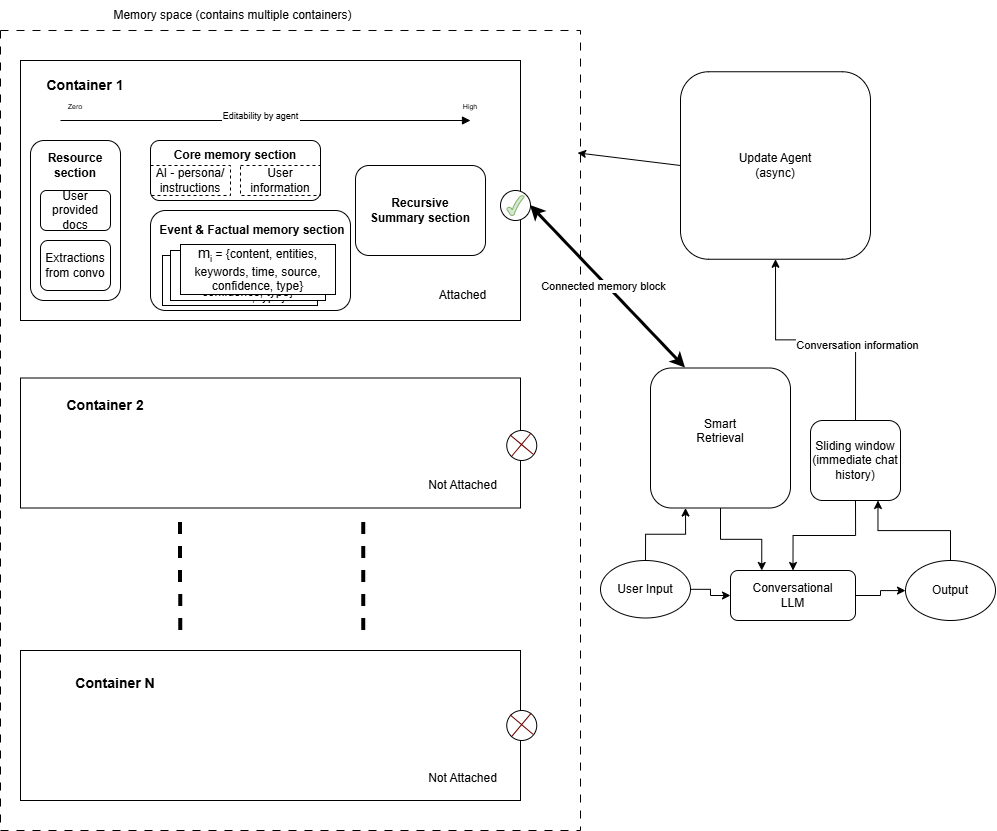
\includegraphics[width=1.1\textwidth]{memBlocks_diagram1.png}
    \caption{MemBlocks System Architecture Overview}
    \label{fig:memBlocks_diagram1}
\end{figure}

\begin{figure}[htbp]
    \centering
    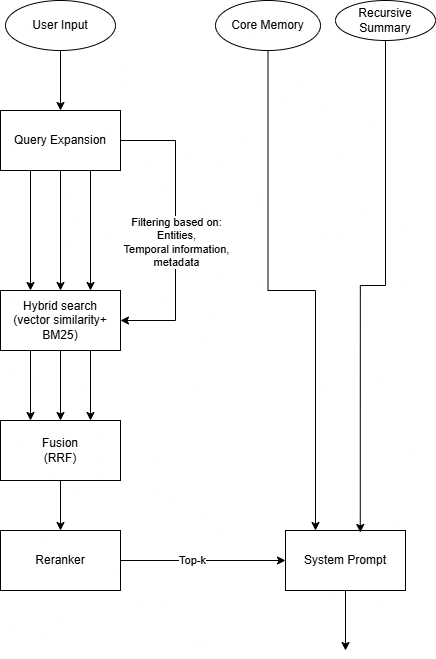
\includegraphics[width=0.8\textwidth]{smart_retriver.png}
    \caption{Smart Retrieval Pipeline}
    \label{fig:smart_retriver}
\end{figure}

\begin{figure}[htbp]
    \centering
    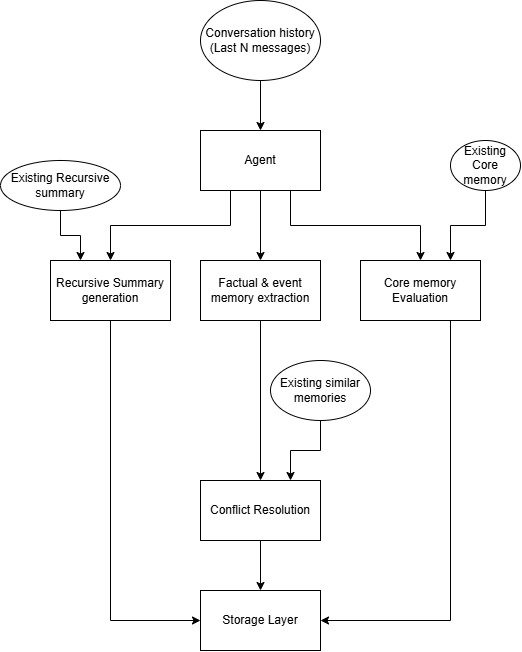
\includegraphics[width=0.8\textwidth]{update_agent.png}
    \caption{Update Agent Pipeline}
    \label{fig:update_agent}
\end{figure}

\begin{figure}[htbp]
    \centering
    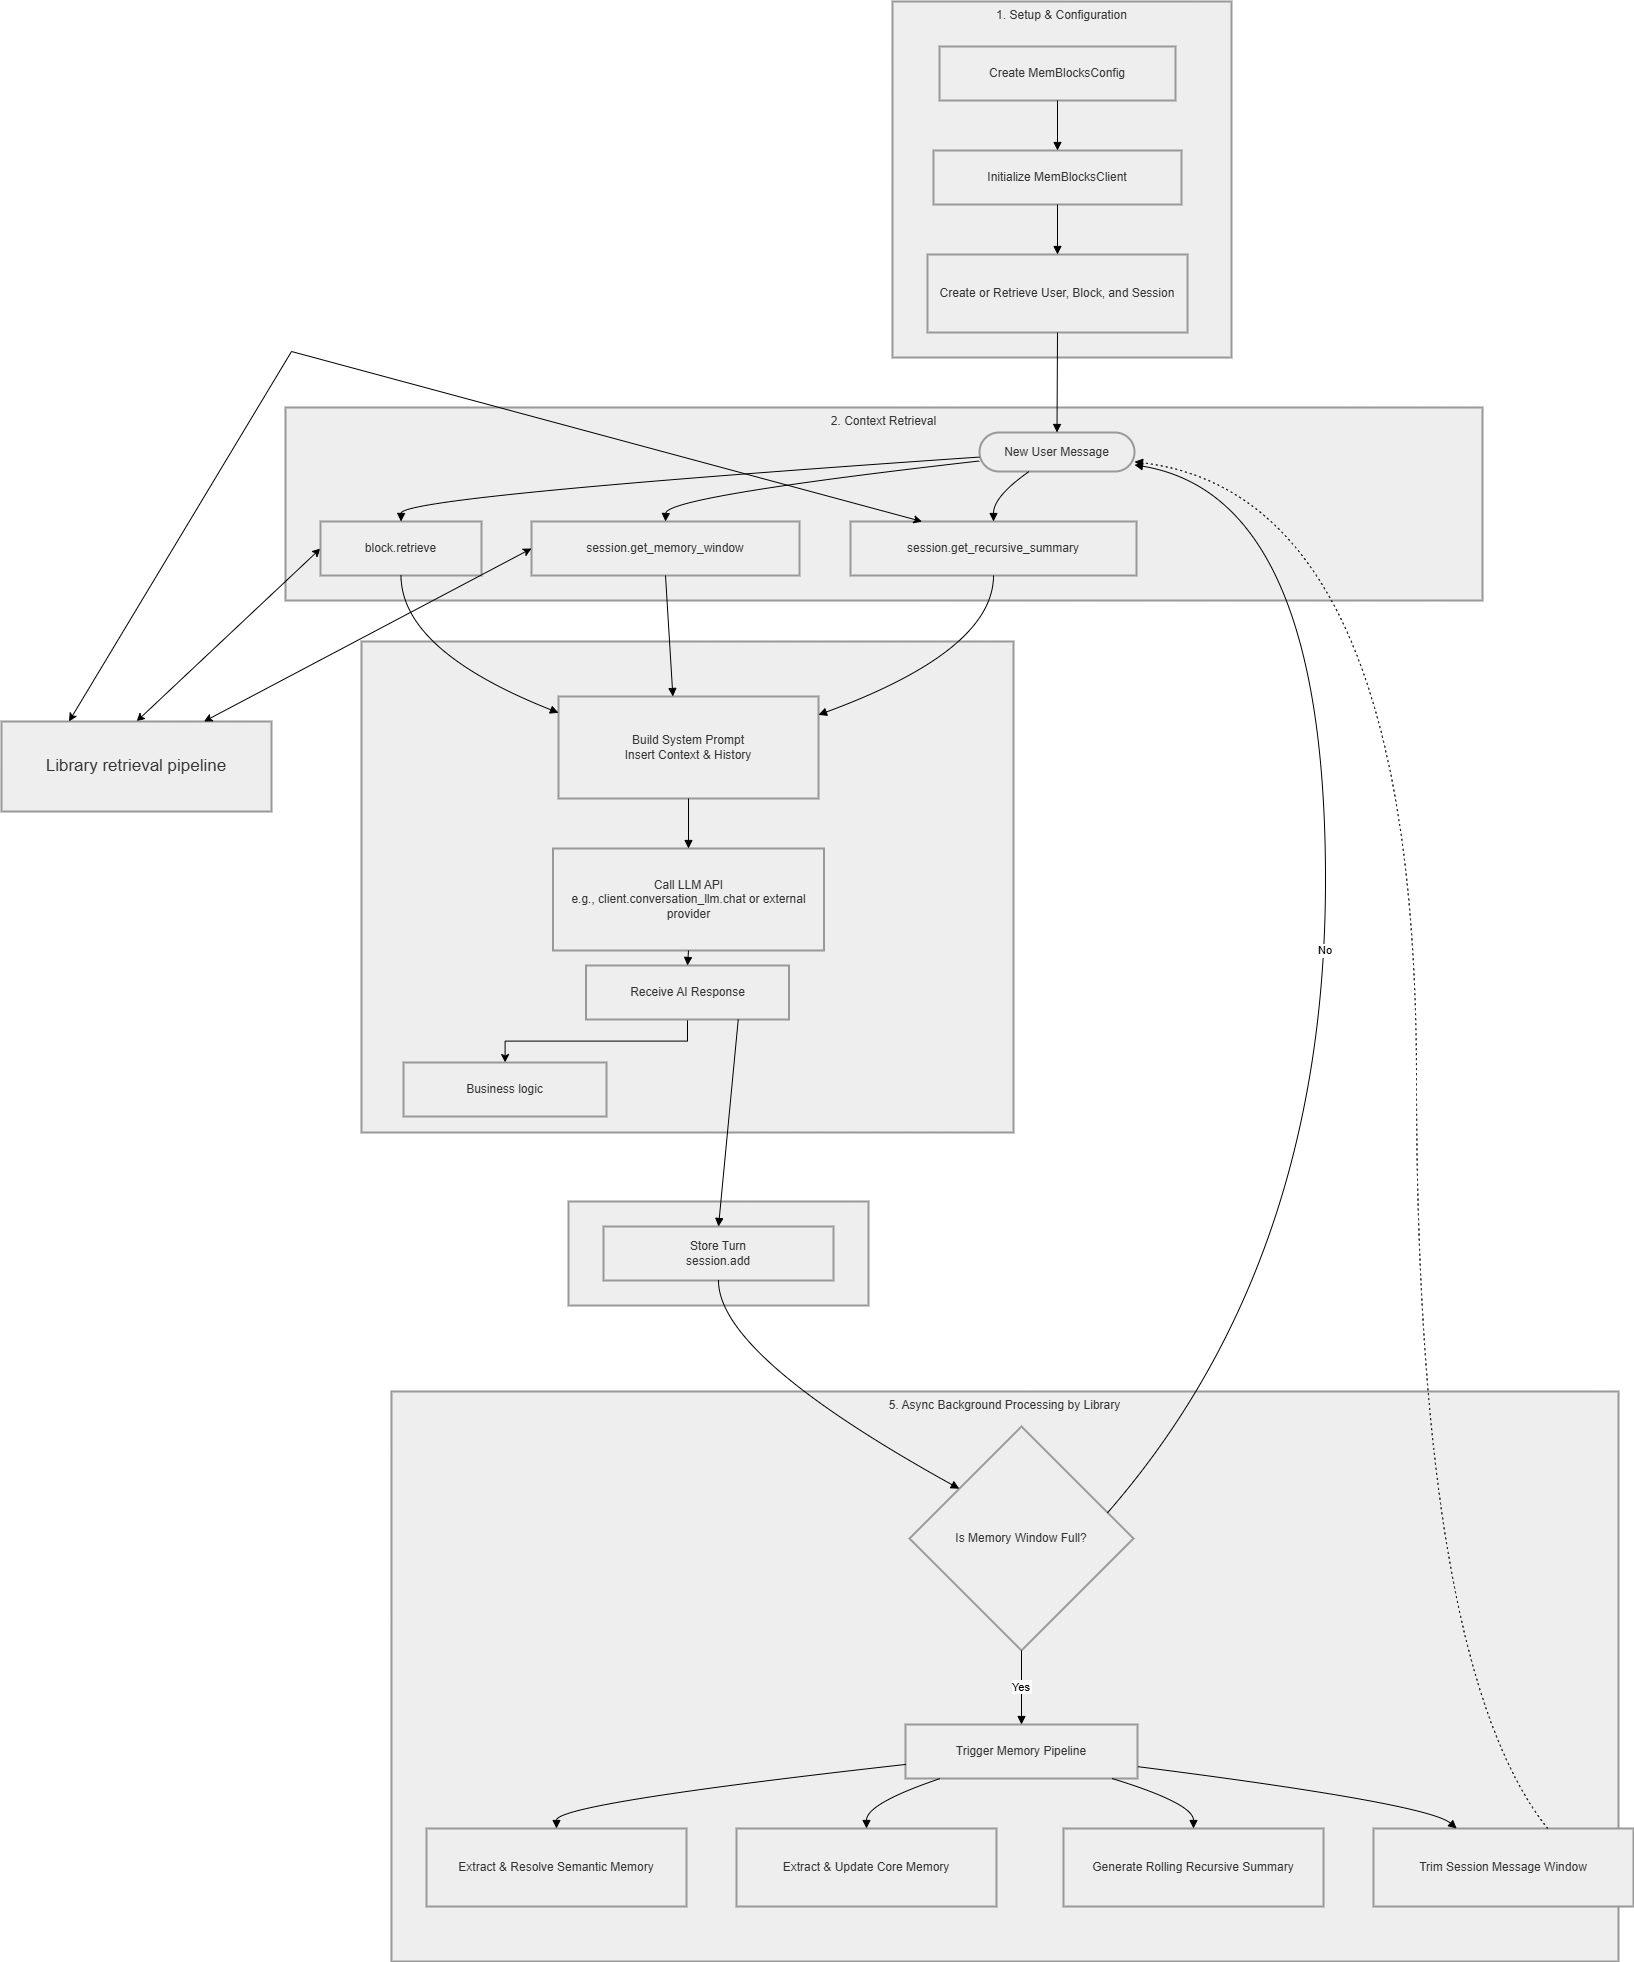
\includegraphics[width=1.0\textwidth]{recommended_userflow.png}
    \caption{Recommended Developer Implementation Flow}
    \label{fig:recommended_userflow}
    
    \vspace{0.5em}
    \small \textbf{Developer Integration Workflow:}\par
    \noindent Figure \ref{fig:recommended_userflow} outlines the recommended lifecycle for integrating the MemBlocks library into an external architecture. It illustrates the progression from client initialization and namespace configuration to the active, low-latency interaction loop where background operations handle memory consolidation asynchronously.
\end{figure}

\begin{figure}[htbp]
    \centering
    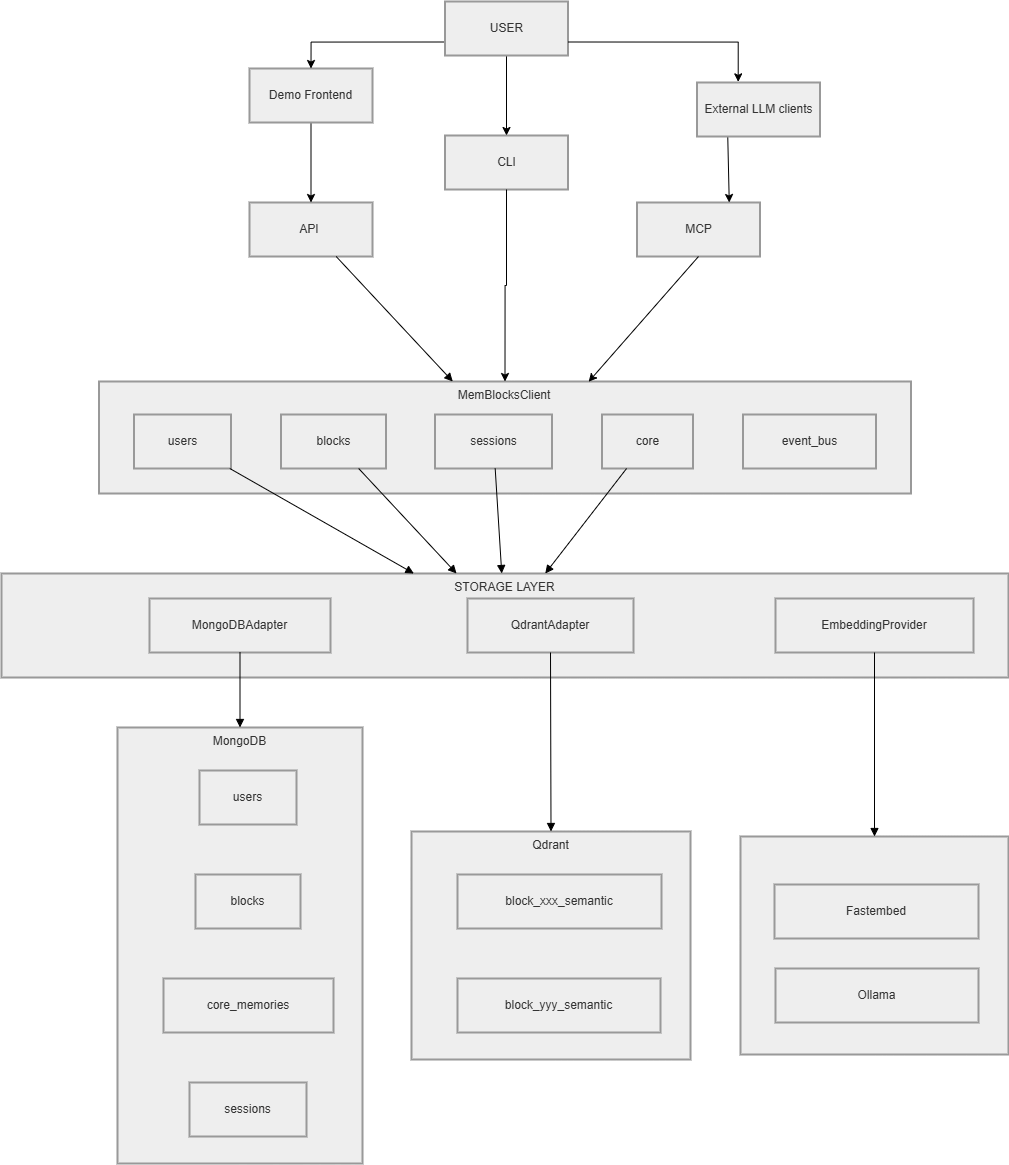
\includegraphics[width=1.0\textwidth]{dataflow.png}
    \caption{MemBlocks Internal Data Flow}
    \label{fig:dataflow}

    \vspace{0.5em}
    \small \textbf{Systems Data Flow:}\par
    \noindent Figure \ref{fig:dataflow} visualizes the journey of user interactions through the MemBlocks pipeline. It highlights the front-end prompt assembly—where isolated context fragments and conversation history are synthesized—and the back-end extraction cycle, illustrating how persistent data stores are updated out of band when sliding window thresholds are met.
\end{figure}

\clearpage

\section{Results and Discussion}

The deployment and testing of the MemBlocks architecture demonstrated a successful resolution of all core functional and structural requirements defined prior to implementation. By evaluating the system's runtime behavior, memory routing integrity, and prompt assembly process, it was confirmed that the modular memory management framework is both practical for deployment and highly effective at stabilizing AI agent context.

\subsection{Fulfillment of System Requirements}

The implemented system successfully satisfied the established design requirements through the following observed capabilities:

\textbf{1. Context Isolation and Dynamic Block Attachment:}\par
Testing verified that memory \texttt{Blocks} operate as strictly independent namespaces. By segregating storage at the block level, the system enforced clear boundaries between different conceptual domains (e.g., separating a user's personal coding projects from general knowledge). The ability to dynamically attach and detach these blocks proved crucial: it ensures that an agent is never distracted by out-of-scope data, a frequent flaw in monolithic vector databases.

\textbf{2. Sectioned Memory Processing and Retrieval:}\par
The architectural split between Core Memory, Semantic Memory, and the Recursive Summary was fully operationalized. Performance tracking indicated that maintaining persistent high-priority facts (Core) while injecting only the top-ranked semantic memories prevented the underlying Language Models from experiencing context bloat. The continuous compression into the Recursive Summary proved adept at bridging the conversational past without retaining unnecessary raw token overhead. 

\textbf{3. Controlled Updates and Conflict Resolution:}\par
One of the most critical operational requirements successfully validated was the system's conflict-aware memory storage. Upon reaching the sliding window threshold, the extraction workflows bypassed naive append-only behavior. Instead, through the Memory Resolution Workflow, new insights were systematically checked against existing memories, resulting in intelligent \texttt{ADD}, \texttt{UPDATE}, and \texttt{DELETE} operations. This capability is vital for preventing duplicated, contradictory records as the agent learns and grows over time.

\subsection{Significance for Agentic AI Systems}

The successful integration of the MemBlocks pipeline represents a necessary evolution in how Large Language Models interact with long-term memory. Traditionally, AI memory has relied on unstructured data dumps (e.g., standard Retrieval-Augmented Generation), which degrade over long interactions through context-window saturation and retrieval hallucinations.

By demonstrating that retrieval and storage can operate as a closed, bidirectional loop, MemBlocks exhibits the type of architectural maturity required for advanced agentic AI. The proactive conflict-resolution algorithms ensure that the database's integrity actively improves over time, rather than passively degrading. Furthermore, the explicit capability to override automated loops---via programmatic event triggers, isolated retrieval, and manual flush commands---provides developers with the precise governance needed over non-deterministic AI behavior. 

Ultimately, MemBlocks moves beyond theoretical design to offer a robust, context-aware foundation. This approach to structured, modular memory is essential for the future deployment of autonomous, multi-domain AI agents running uninterrupted across complex problem spaces.

\section{Conclusion}

The MemBlocks project was initiated to resolve a fundamental bottleneck in the deployment of autonomous AI agents: the degradation of reasoning caused by unstructured, infinitely compounding context windows. By transitioning away from monolithic vector databases toward a structured, sectioned memory architecture, this project successfully demonstrated that an LLM's operational memory can be both modular and highly controllable.

Through the implementation of independent memory \texttt{Blocks}, distinct storage sections (Core, Semantic, Recursive Summary), and background extraction workflows, the system successfully shields the active prompt from irrelevant noise while ensuring high-fidelity recall. Most critically, the transition from append-only storage to a conflict-aware resolution pipeline ensures that the agent's memory base refines and self-corrects over time, establishing a reliable foundation for long-term user interaction. The resulting library and MCP integration prove that advanced memory orchestration can be seamlessly integrated into modern Agentic pipelines without compromising response latency or data integrity.

\section{Limitations and Future Enhancements}

While the initial implementation of the MemBlocks architecture successfully resolves the core issues of context-bloat and memory routing, there are several avenues for future research and capability expansion:

\textbf{1. Resource Ingestion Pipeline:}\par
Currently, the pipeline processes explicit conversational turns via the Semantic and Core extraction workflows. However, the architectural design explicitly reserves a \texttt{Resource Section} for handling dense, external documents (e.g., PDFs, code repositories). A primary future enhancement will involve building ingestion pipelines to attach these static documents to specific Blocks, allowing the hybrid retrieval mechanics to seamlessly blend dynamic dialogue facts with grounded document citations.

\textbf{2. Graph-Aware Conflict Resolution:}\par
The current conflict resolution mechanism safely handles localized paradoxes (e.g., updating a user's favorite language from Python to Rust). However, as memory repositories grow, related facts become deeply intertwined. Future iterations should explore multi-pass or knowledge-graph-aware conflict handling, where updating a single fundamental fact automatically propagates updates to downstream dependent memories without requiring exhaustive, brute-force vector scans.

\textbf{3. Multi-Agent Shared Context:}\par
The current namespace isolation is optimized for single-agent-to-user dynamics. An exciting direction for enhancement is extending the `Block` ownership model to support robust multi-agent orchestration, where different specialized agents can concurrently read from and write to shared memory blocks with conflict-locking mechanisms.

\section{Appendix}

\textbf{Project Repository:} \url{https://github.com/Ashish-Pandey62/MemBlocks}

\subsection{Prompt Artifacts}

\begin{itemize}
    \item \texttt{PS1\_SEMANTIC\_PROMPT}: \texttt{memblocks\_lib/src/memblocks/prompts/\_\_init\_\_.py}, line 10.
    \item \texttt{PS2\_MEMORY\_UPDATE\_PROMPT}: \texttt{memblocks\_lib/src/memblocks/prompts/\_\_init\_\_.py}, line 297.
\end{itemize}

\subsection{Core Data Models}

\textbf{Memory block metadata and block structure.}
\begin{itemize}
    \item \texttt{MemoryBlockMetaData}: \texttt{memblocks\_lib/src/memblocks/models/block.py}, line 22.
    \item \texttt{MemoryBlock}: \texttt{memblocks\_lib/src/memblocks/models/block.py}, line 45.
\end{itemize}

\textbf{Section and LLM output models.}
\begin{itemize}
    \item \texttt{SemanticMemoryData}: \texttt{memblocks\_lib/src/memblocks/models/memory.py}, line 17.
    \item \texttt{CoreMemoryData}: \texttt{memblocks\_lib/src/memblocks/models/memory.py}, line 32.
    \item \texttt{ResourceMemoryData}: \texttt{memblocks\_lib/src/memblocks/models/memory.py}, line 47.
    \item \texttt{SemanticExtractionOutput}: \texttt{memblocks\_lib/src/memblocks/models/llm\_outputs.py}, line 10.
\end{itemize}

\subsection{API Request Models}

\textbf{Backend request contracts.}
\begin{itemize}
    \item \texttt{CreateBlockRequest}: \texttt{backend/src/api/models/requests.py}, line 11.
    \item \texttt{ChatRequest}: \texttt{backend/src/api/models/requests.py}, line 25.
    \item \texttt{SearchMemoriesRequest}: \texttt{backend/src/api/models/requests.py}, line 34.
\end{itemize}

\clearpage

\bibliographystyle{IEEEtran}
\bibliography{references}

\end{document}
